% Template for PLoS
% Version 3.1 February 2015
%
% To compile to pdf, run:
% latex plos.template
% bibtex plos.template
% latex plos.template
% latex plos.template
% dvipdf plos.template
%
% % % % % % % % % % % % % % % % % % % % % %
%
% -- IMPORTANT NOTE
%
% This template contains comments intended 
% to minimize problems and delays during our production 
% process. Please follow the template instructions
% whenever possible.
%
% % % % % % % % % % % % % % % % % % % % % % % 
%
% Once your paper is accepted for publication, 
% PLEASE REMOVE ALL TRACKED CHANGES in this file and leave only
% the final text of your manuscript.
%
% There are no restrictions on package use within the LaTeX files except that 
% no packages listed in the template may be deleted.
%
% Please do not include colors or graphics in the text.
%
% Please do not create a heading level below \subsection. For 3rd level headings, use \paragraph{}.
%
% % % % % % % % % % % % % % % % % % % % % % %
%
% -- FIGURES AND TABLES
%
% Please include tables/figure captions directly after the paragraph where they are first cited in the text.
%
% DO NOT INCLUDE GRAPHICS IN YOUR MANUSCRIPT
% - Figures should be uploaded separately from your manuscript file. 
% - Figures generated using LaTeX should be extracted and removed from the PDF before submission. 
% - Figures containing multiple panels/subfigures must be combined into one image file before submission.
% For figure citations, please use "Fig." instead of "Figure".
% See http://www.plosone.org/static/figureGuidelines for PLOS figure guidelines.
%
% Tables should be cell-based and may not contain:
% - tabs/spacing/line breaks within cells to alter layout or alignment
% - vertically-merged cells (no tabular environments within tabular environments, do not use \multirow)
% - colors, shading, or graphic objects
% See http://www.plosone.org/static/figureGuidelines#tables for table guidelines.
%
% For tables that exceed the width of the text column, use the adjustwidth environment as illustrated in the example table in text below.
%
% % % % % % % % % % % % % % % % % % % % % % % %
%
% -- EQUATIONS, MATH SYMBOLS, SUBSCRIPTS, AND SUPERSCRIPTS
%
% IMPORTANT
% Below are a few tips to help format your equations and other special characters according to our specifications. For more tips to help reduce the possibility of formatting errors during conversion, please see our LaTeX guidelines at http://www.plosone.org/static/latexGuidelines
%
% Please be sure to include all portions of an equation in the math environment.
%
% Do not include text that is not math in the math environment. For example, CO2 will be CO\textsubscript{2}.
%
% Please add line breaks to long display equations when possible in order to fit size of the column. 
%
% For inline equations, please do not include punctuation (commas, etc) within the math environment unless this is part of the equation.
%
% % % % % % % % % % % % % % % % % % % % % % % % 
%
% Please contact latex@plos.org with any questions.
%
% % % % % % % % % % % % % % % % % % % % % % % %

\documentclass[10pt,letterpaper]{article}
\usepackage[top=0.85in,left=2.75in,footskip=0.75in]{geometry}

% Use adjustwidth environment to exceed column width (see example table in text)
\usepackage{changepage}

% Use Unicode characters when possible
\usepackage[utf8]{inputenc}

% textcomp package and marvosym package for additional characters
\usepackage{textcomp,marvosym}

% fixltx2e package for \textsubscript
\usepackage{fixltx2e}

% amsmath and amssymb packages, useful for mathematical formulas and symbols
\usepackage{amsmath,amssymb}

% cite package, to clean up citations in the main text. Do not remove.
\usepackage{cite}

% Use nameref to cite supporting information files (see Supporting Information section for more info)
\usepackage{nameref,hyperref}

% line numbers
\usepackage[right]{lineno}

\usepackage{graphicx} 

\usepackage{amssymb}
\usepackage{bm}
% \graphicspath{{./figures/}} % save all figures in the same directory

\newcommand{\given}{\mid}
\newcommand{\me}{\mathrm{e}} % use for base of the natural logarithm
\newcommand{\md}{\mathrm{d}} % use for base of the natural logarithm
\newcommand{\mean}{\mathrm{E}}
\newcommand{\Normal}{\mathcal{N}}
\newcommand{\argmax}{\operatornamewithlimits{argmax}}
\newcommand{\like}{\mathcal{L}}

% ligatures disabled
\usepackage{microtype}
\DisableLigatures[f]{encoding = *, family = * }


\usepackage{bm}
% rotating package for sideways tables
\usepackage{rotating}

% Remove comment for double spacing
%\usepackage{setspace} 
%\doublespacing

% Text layout
\raggedright
\setlength{\parindent}{0.5cm}
\textwidth 5.25in 
\textheight 8.75in

% Bold the 'Figure #' in the caption and separate it from the title/caption with a period
% Captions will be left justified
\usepackage[aboveskip=1pt,labelfont=bf,labelsep=period,justification=raggedright,singlelinecheck=off]{caption}

% Use the PLoS provided BiBTeX style
\bibliographystyle{plos2015}

% Remove brackets from numbering in List of References
\makeatletter
\renewcommand{\@biblabel}[1]{\quad#1.}
\makeatother

% Leave date blank
\date{}

% Header and Footer with logo
\usepackage{lastpage,fancyhdr,graphicx}
\nonstopmode  % to allow pdflatex to compile even if errors are raised (e.g. missing figures)
\usepackage{epstopdf}
\pagestyle{myheadings}
\pagestyle{fancy}
\fancyhf{}
\lhead{
\includegraphics[width=2.0in]{PLOS-submission.eps}}
\rfoot{\thepage/\pageref{LastPage}}
\renewcommand{\footrule}{\hrule height 2pt \vspace{2mm}}
\fancyheadoffset[L]{2.25in}
\fancyfootoffset[L]{2.25in}
\lfoot{\sf PLOS}

%% Include all macros below

\newcommand{\lorem}{{\bf LOREM}}
\newcommand{\ipsum}{{\bf IPSUM}}

%% END MACROS SECTION


\begin{document}
\vspace*{0.35in}

% Title must be 250 characters or less.
% Please capitalize all terms in the title except conjunctions, prepositions, and articles.
\begin{flushleft}
{\Large
\textbf\newline{Matrix Ash}
}
\newline
% Insert author names, affiliations and corresponding author email (do not include titles, positions, or degrees).
\\
Sarah Urbut \textsuperscript{1,2},
Gao Wang {1},
%Name3 Surname\textsuperscript{2,\textcurrency a},
%Name4 Surname\textsuperscript{2,\ddag},
%Name5 Surname\textsuperscript{2,\ddag},
%Name6 Surname\textsuperscript{2},
Matthew Stephens \textsuperscript{1,3,\ddag},
with the GTEX Consortium\textsuperscript{\textpilcrow}
\\
\bigskip
\bf{1} Department of Human Genetics/ University of Chicago, Chicago, IL USA
\\
\bf{2} Pritzker School of Medicine/Growth and Development Training Program/University of Chicago, Chicago, IL USA
\\
\bf{3} Department of Statistics/ University of Chicago, Chicago, IL USA

\\
\bigskip

% Insert additional author notes using the symbols described below. Insert symbol callouts after author names as necessary.
% 
% Remove or comment out the author notes below if they aren't used.
%
% Primary Equal Contribution Note
%\Yinyang These authors contributed equally to this work.

% Additional Equal Contribution Note
% Also use this double-dagger symbol for special authorship notes, such as senior authorship.
%\ddag These authors also contributed equally to this work.

% Current address notes
%\textcurrency a Insert current address of first author with an address update
% \textcurrency b Insert current address of second author with an address update
% \textcurrency c Insert current address of third author with an address update

% Deceased author note
%\dag Deceased

% Group/Consortium Author Note
%\textpilcrow Membership list can be found in the Acknowledgments section.

% Use the asterisk to denote corresponding authorship and provide email address in note below.
%* CorrespondingAuthor@institute.edu

\end{flushleft}
% Please keep the abstract below 300 words
\section*{Abstract}
%Lorem ipsum dolor sit amet, consectetur adipiscing elit. Curabitur eget porta erat. Morbi consectetur est vel gravida pretium. Suspendisse ut dui eu ante cursus gravida non sed sem. Nullam sapien tellus, commodo id velit id, eleifend volutpat quam. Phasellus mauris velit, dapibus finibus elementum vel, pulvinar non tellus. Nunc pellentesque pretium diam, quis maximus dolor faucibus id. Nunc convallis sodales ante, ut ullamcorper est egestas vitae. Nam sit amet enim ultrices, ultrices elit pulvinar, volutpat risus.


% Please keep the Author Summary between 150 and 200 words
% Use first person. PLOS ONE authors please skip this step. 
% Author Summary not valid for PLOS ONE submissions.   
\section*{Author Summary}
Variation in gene expression is an important mechanism underlying susceptibility to complex disease.  The simultaneous genome-wide assay of gene expression and genetic variation allows the mapping of the genetic factors that underpin individual differences in quantitative levels of expression (expression QTLs; eQTLs). 
By analyzing these effects across multiple tissues, we exploit the information that the effect of the gene-snp pair in one tissue can provide about its effect in alternative tissues.
Furthermore, quantifying the effect size as opposed to simply calling QTLs present or absent reveal many patterns of sharing of effects among tissues which differ in both sign and magnitude.
We provide a novel framework for estimating effect sizes across multiple subgroups, considering the evidence contained in all subgroups jointly, which provides a powerful and detailed insight into quantitative heterogeneity present in the genome.

%The availability of systematically generated eQTL information could provide immediate insight into a biological basis for disease associations identified through genome-wide association (GWA) studies, and can help to identify networks of genes 
%involved in disease pathogenesis (\cite{nicolae_trait-associated_2010, veyrieras_high-resolution_2008}). However, most studies to date have been conducted in a single immortalized peripheral cell type, and it is unclear to what extent these findings will translate to human disease mapping across more varied cell types. 
%Furthermore, even analyses performed on additional cell types are often performed in a single tissue framework \cite{majewski_study_2011,gilad_revealing_2008} and fail to correlate the effect of genetics across multiple tissue types.  The Genotype Tissue Expression Project, GTEx, Project will provide the data necessary to address this situation: by 2016, the resource is expected to enroll a total of approximately 900 post-mortem donors, with approximately 30 tissues collected from each donor, and the project
%will generate extensive genotype data and RNA-seq data on each individual. However,  available methods are limited in their ability to {\it jointly analyze data on all tissues} to maximize power, while
%simultaneously {\it allowing for both qualitative and quantitative differences among eQTLs} present in each tissue.



\linenumbers

\section*{Introduction}
Variation in gene expression is an important mechanism underlying susceptibility to complex disease.The simultaneous genome-wide assay of gene expression and genetic variation allows the mapping of the genetic factors that underpin individual differences in quantitative levels of expression (expression QTLs; eQTLs). 
The availability of this information provides immediate insight into a biological basis for disease associations identified through genome-wide association (GWA) studies, and can help to identify networks of genes 
involved in disease pathogenesis (\cite{nicolae_trait-associated_2010, veyrieras_high-resolution_2008}).
Available methods are limited not only in their ability to {\it jointly analyze data on all tissues} to maximize power, but also in simultaneously {\it allowing for both qualitative and quantitative differences among eQTLs} present in each tissue.

Initial approaches to quantify the effect of a particular SNP on gene expression considered only one tissue at a time, and ignored the effect of the SNP on gene expression in other tissues.
This fails to exploit the power of  shared genetic variation in effects on expression - i.e. the information that the effect of the gene-snp pair in one tissue can provide about the effect in another- and limits our understanding of multiple-tissue phenotypes.
Furthermore, even past attempts at quantifying heterogeneity of eQTLs using the data across tissues jointly were limited in both the number of tissues considered, and also the level of heterogeneity considered. Qualitative heterogeneity refers to calling a snp `active' or `inactive' in a given tissue. For example, previous attempts at joint analyses referred to the setting in which the gene-snp pair is active in all tissues as `shared' and active in only one as `tissue-specific'  (\cite{flutre_statistical_2013,wen_bayesian_2014}).
However, a QTL may be `active' in all or many tissues and with varying magnitude or sign; we refer to this as quantitative heterogeneity.

Thus, the novel approach we offer here allows groups of QTLs to be classified not only by their presence or absence in a particular tissue, but by their relationships in continuous effects between tissues, e.g., consistently larger effects in some tissues than other.
 Indeed, our initial motivation came from our group's past analysis of GTEx pilot data \cite{consortium_genotype-tissue_2015}, in which we saw evidence that many $(50\%)$ QTLs are shared across all nine tissues. In this context, a QTL was called based on whether it demonstrates significant posterior probability of being active in a particular tissue. Applying our hierarchical model to the dataset from Dimas {\it et al} \cite{dimas_common_2009} with 3 tissues, we found just 8\% of eQTLs are specific to a single tissue, with an estimated 88\% of eQTLs being common to fibroblasts, LCL cells and T-Cells \cite{flutre_statistical_2013}. Not all eQTLs are shared by all tissues; some tissues may share eQTLs more than others. To allow for this, our previous hierarchical model attempted to infer the extent of such sharing by estimating the proportion of eQTL which were shared in various `configurations' or patterns of binary activity in which a QTL was `called' or `absent' in each tissue.
 However, these binary configurations are still \textit{limited in their ability to capture continuous variation} in levels of activity among tissues in which the SNP is considered active. 
 In fact, as the number of tissues considered increases, perhaps the more interesting and biologically relevant question becomes one of quantitative heterogeneity - that is, how do the patterns of effect vary across tissues in which the SNP is called `active'.  
Critically, quantifying the effect sizes of the gene-snp pair across tissues considering the evidence contained in all tissues jointly thus reveals new patterns of activity across tissues, which differ in their relationship in sign and magnitude within and between tissues. Thus effects can be `shared' but not `consistent' across tissues. The structure of this paper is as follows: we will describe our approach in brief for modeling and estimating these effect sizes across tissues, demonstrate the utility of such an approach on simulated data, and apply our method to data from the GTEX dataset, version 6.0, where we analyze effects size for 16,069 genes across 44 tissues. In so doing, offer novel insight into the patterns of quantitative heterogeneity in genetics effects among a greater number of tissues than ever analyzed before.

\subsection{Methods Overview: Approach} 

We aim to learn about patterns of sharing across tissues within a SNP and among SNPs, which join to help us better understand the global and snp-specific patterns of effects of genetics on gene expression. 
This allows us to make comparisons among tissues in which the QTL is called active, and among gene-snp pairs with a similar degree of activity in a given tissue. 
Thus as an additional level of combining information, we assume that each eQTL may follow a particular pattern of activity characterized by its effects across tissues. Within these groups, the tissues exhibit characteristic patterns of sharing, which can be captured by considering the covariance structure of the genetic effects among tissues. 

This lends itself to a mixture model, in which  we assume all the gene-snp pairs arise from a mixture of a finite number of multivariate normal (MVN) distribution, each characterized by the covariance matrix from which the vector of effects is though to arise. For each of $\textbf{J}$ gene-snp pairs, we observe an R dimensional vector of standardized effect sizes %$\bm{\hat{b}}$
and their standard error and assume that these effects descend from some true effect size $\bm{b}$. 



 \begin{equation}
  \bm{b_{j}} | \bm{\pi},\bf{U} \sim \sum_{k,l} \pi_{k,l} \;{\it N}_R(.;\bm{0}, \omega_l U_{k})
  \label{eqn:mixprior}
\end{equation}

Here, the covariance matrix $U_{k}$ captures the particular patterns of sharing reflecting the variation in effect sizes within and between tissues, while $\omega_{l}$ determines the scale of each pattern - the magnitude of the effect size. The relationship among the distinct entries of this matrix allows us to specify effects which may be consistently larger in some tissues relative to others and may possess variable correlation among different pairs of tissues (e.g., see Figure \ref{fig:Patterns}, \textbf{B}, for converse relationships among effects in tissue one and two for SNPs of green opposed to blue class). Thus we also recognize that while two eQTL may obey a similar pattern or shape, the absolute scale may vary. For example, two eQTL may both have strong correlation between liver and lung with consistently larger effects in liver, but the absolute size of the effects may vary between SNPs (Figure \ref{fig:Patterns}, \textbf{A}, contrast gene-snp pairs of far left and far right pattern).\newline

%\textbf{Figure: Colorful patterns, caption indicates different patterns of activity across tissues in groups 1-3, same pattern or shape for snps of group 4 but tendency towards small effects}

\newline
\begin{figure}[htbp]
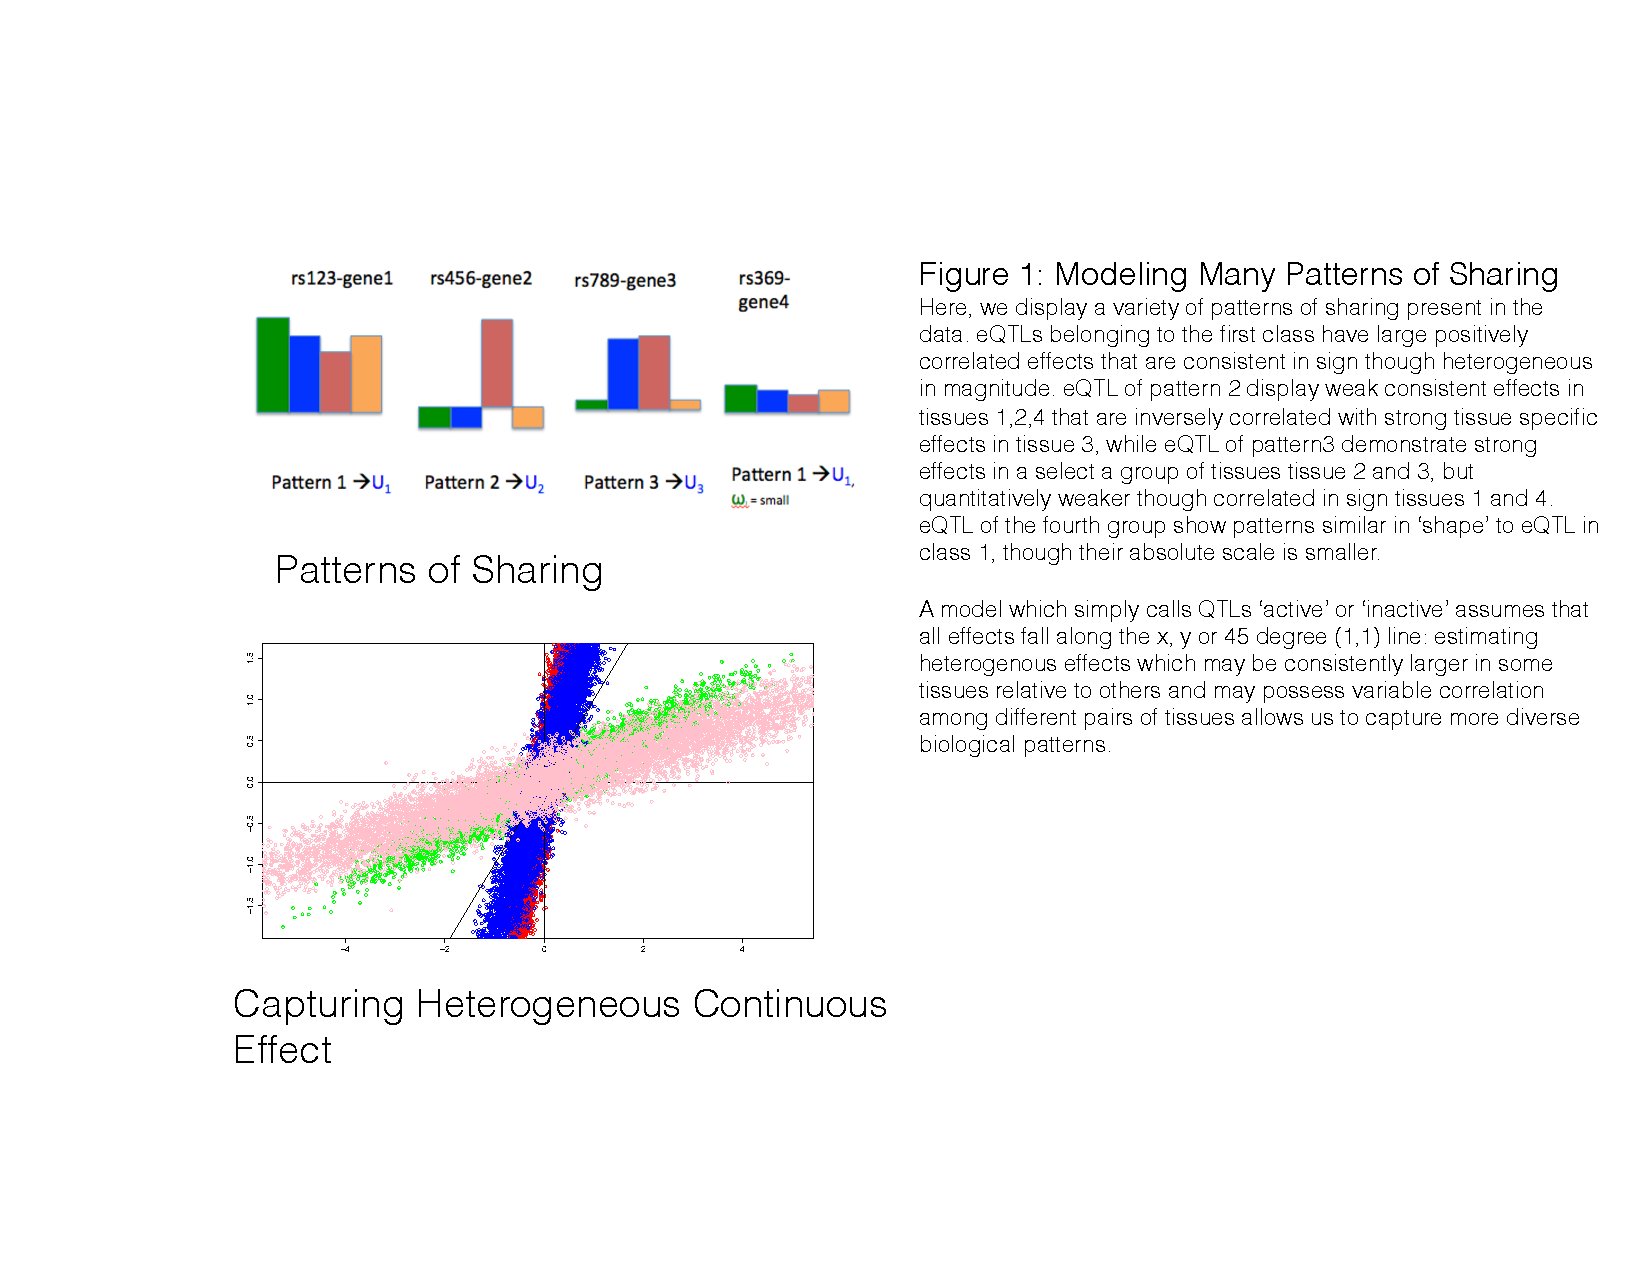
\includegraphics[width=10cm]{Figures/Patterns.pdf}
\caption{\textbf{Modeling Many Patterns of Sharing.} \textbf{A:} Here, we display a variety of patterns of sharing present in the data. eQTLs belonging to the first class have large positively correlated effects that are consistent in sign though heterogeneous in magnitude. eQTL of pattern 2 display weak consistent effects in liver, lung and thyroid that are inversely correlated with strong tissue specific effects in brain, while eQTL of pattern 3 demonstrate strong effects in a select a group of tissues (here, lung and brain), but quantitatively weaker though correlated in sign with liver and thyroid. eQTL of the fourth group show patterns similar in `shape' to eQTL in class 1, though their absolute scale is smaller. \textbf{B:} In this two tissue-example, a model which simply calls QTLs `active' or `inactive' assumes that all effects fall along the x, y or 45 degree (1,1) line: estimating heterogenous effects which may be consistently larger in some tissues relative to others and may possess variable correlation among different pairs of tissues allows us to capture more diverse biological patterns.}
\label{fig:Patterns}
\end{figure}
\newline


\subsection{Previous Approach}
 
Previous work from our lab considered the idea of configuration - i.e., that a tissue was simply `active' or `inactive' in a particular tissues - and thus for R tissues, there were $2^{R}$ possible configurations, which becomes computationally infeasible as $R$ grows. Thus a non-trivial novelty of our approach is its application to joint estimation of effects across a larger number of $R$= 44 tissues, never before described.

Furthermore, this considered only the idea that the variance in effect sizes between two tissues was the same across tissues thought to be active and the covariances were also the same among tissues thought to be active in a given `configuration',  and thus failed to incorporate the much richer covariance structure between tissues. For example, many gene-SNP pairs might follow a pattern in which it is common to be `active' across all tissues, but some QTL may have consistently larger effects in liver, lung and thyroid while other QTL may possess consistently larger effects in brain tissues and still another class of gene-snp pairs may show consistently quantitatively specific activity in whole blood but non-trivial effects in other tissues. 

As a critical innovation on our previous work \cite{flutre_statistical_2013,wen_bayesian_2014} the covariance matrices used here contain distinct diagonal and off-diagonal elements which reflect data-specific patterns of variation within and covariance between subgroups (tissues). This captures the variation in effect sizes within and between subgroups better than restricting effects to simply `shared' or `unshared'. This effectively amounts to a random effects analysis in which we assume that the between subgroup variability, here the entries of the matrix $U_{k}$ is unique for each study (see Borenstein et al).

Because we can't know the `true covariance matrix' for each gene-snp pair, we aim to assemble a list which sufficiently captures the various patterns, and then `learn' the relative proportions of each pattern of sharing from the data. One can now model each vector of effect sizes $\bm{b_{j}}$ as arising from a mixture that captures all the covariance patterns present (Equation \ref{eqn:mixprior}).

The primary novelty of this approach is {\it to estimate this multivariate posterior distribution on the effect size in a data-sensitive way} - i.e., using the mixture model to capture information about the covariance structure among subgroups (here, tissues), and thus describe the heterogeneity of effects across tissues, rather than simply calling effects `shared' or `specific'. We deem this model `hierarchical' because these prevailing patterns of activity are learned from the larger dataset - e.g., a large, random set of gene-snp pairs - and influence our inference about a given gene-snp pair `$\bf{j}$'. Thus we might identify a situation in which it is common to have large effects in certain tissues and not others. Accordingly, if a given observed gene-snp pair demonstrates a small effect in one of the `off issues', we might be inclined to conclude that it is indeed a member of this particular class and shrink the small effect in this tissue accordingly without reducing our estimates of the more `active tissues'. However, if we observe the same small effect in a setting in which `similar tissues' have large effects, we might `shrink' this effect size less, due to our high prior belief in the SNP's effectiveness garnered from adjacent tissues. Thus we deem this method `Adaptive Shrinkage' because the appropriate amount of shrinkage is learned from the overall dataset. Critically, our method is dually adaptive, in the sense that we learn the relative abundance of effect sizes and directions from the overarching data set: observed effects are nudged towards prevailing patterns and sizes, according to the learned proportions of each.

Because our prior belief in consistency is strong in this particular dataset, we identify many more `significant associations'  in settings where perhaps the observed univariate statistic in one tissue is small but otherwise large in additional tissues, nudging these effects towards something more consistent. This is in contrast to a univariate shrinkage approach, in which all effects of the same size would be `shrunk' equivalently, due to lack of information garnered from adjacent tissues. 
%
%In fact, shrinkage towards $\bm{0}$ of small effects is a result, not a necessity - since the majority of the prior weight is on small $\omega$ components which emphasize components with small prior variance of the effect size $\textbm{b}$, many of the modest observed effects will be smoothed or shrunk towards the prior mean, $\bm{0}$. 

Critically, in learning about the effect size of a gene-snp pair in each tissue, we can make statements about the degree of heterogeneity present in the data-set: that is the proportion of SNPs who exhibit effects that vary in magnitude or sign. Conversely, we can describe the degree of homogeneity should these phenomena be rare. Thus we offer an additional description to eQTL analysis: the degree of heterogeneity across multiple subgroups in both sign and magnitude, by characterizing a particular QTL by the similarity in size of its effects across subgroups. 

\section*{Materials and Methods}

Let  $\bm{b_{j}}$ represents the genetic effect of SNP-gene pair $j$ across $R$ = 44 tissues.

We assume the following mixture prior for the $R$ dimensional vector of true effects,  

 \begin{equation}
  \bm{b_{j}} | \bm{\pi},\bf{U}, \bm{\omega} \sim \sum_{k,l} \pi_{k,l} \;{\it N}_R(x; \bm{0}, \omega_l U_{k})
\end{equation}

Where ${\it N}_R(.; \bm{0}, \omega_l U_{k})$ denotes the density of a normal distribution with mean $\bm{0}$ and variance $\omega_l U_{k}$.


%As mentioned above, 
Each component of the mixture distribution is characterized by these prior covariance matrices, $U_{k}$ which capture the pattern of effects across tissues. Critically, this prior distribution is the same for all $J$ - hence the hierarchical incorporation of shared information.

\subsection{ Covariance Matrices}

For a given $\omega_{l}$, we specify 4 `types' of $RxR$ prior covariance matrices $U_{k,l}$.
\begin{enumerate}

\item $U_{k=1,l}$ = $\omega_l$ $\mathbf{I}_{R}$

\item $U_{k=2,l}$ = $\omega_l$X_{z}$ The (naively) estimated tissue covariance matrix as estimated from the column-centered J \times R$ matrix of $Z$ statistics, $Z_{center}$: $\frac{1}{J}$ $Z_{center}$^{t}$ $Z_{center}$

\item $U_{k=3,l}$ = $\omega_l$ $\frac{1}{J}$ $V_{1...p}$ $d^{2}_{1...p}$   $V^{t}_{1..p}$ is the rank $p$ eigenvector approximation of the tissue covariance matrices, i.e., the sum of the first $p$ eigenvector approximations, where $\pcv_{1...p}$  represent the eigenvectors of the covariance matrix of tissues and $\pcd_{1...p}$ are the first $p$ eigenvalues.

\item $U_{k=4:4+Q-1,l}$ = $\frac{1}{J}(($\Lambda\mathbf{F})^{t} \Lambda \mathbf{F})_{q}$ corresponding to the $q_{th}$ sparse factor representation of the tissue covariance matrix %(not the sum of the first $q$, as above)

\item $U_{k=4+Q,l}$ = $\frac{1}{J}$ ($\($\Lambda \mathbf{F})^{t} \Lambda \mathbf{F}$ is the sparse factor representation of the tissue covariance matrix, estimated using all $q$ factors.



\item $U_{k=5+Q:R+4+Q,l}$ = $\frac{1}{J}$ $([1 0 0 . . ]'[1 0 0  . . .])$ %is the sparse factor representation of the tissue covariance matrix, estimated using all $q$ factors.
\item $U_{k=R+5+Q,l}$ = $\frac{1}{J}$ $([1 1 1 . . .]'[1 1 1 . . .])$
\item $[1 0 0 0 ...]$ or $[1 1 1  ...]$ represent configurations such that given membership,$\bm{b_{j}}$ arise from the same prior variance.
\end{itemize}

Critically, the computations above are estimated using the strongest snp per gene as characterized by the maximum absolute value across R tissues, in order to optimally initialize a `denoised' matrix of the true effects. 


\subsection{Deconvolution}
To retrieve a `denoised' or `deconvoluted' estimate of the non-single rank dimensional reduction matrices, we then perform deconvolution after initializing the EM algorithm with  the matrices specified in (2), (3) and (5). The final results of this iterative procedure preserves the rank of the initialization matrix, and allows us to use the `true' effect at each component component $\bm{{b}_{j}}$ as missing data in deconvoluting the prior covariance matrices. In brief, this algorithm works by treating not only the component identity but also the true effect $\bm{{b}_{j}}$  as unobserved data, and maximizing the likelihood over the expectation of the complete data likelihood, considering the values $\bm{{b}_{j}}$ as extra missing data (in addition to the indicator variables $q_{ij}$) (Bovy et al, 2014). 
%
%This allows us to write down the `full data' log likelihood as follows:
%
%\begin{equation}
%\begin{center}
%\begin{aligned}
%\phi=\sum_{J} \sum_{K} q_{jk} ln \alpha_{k} \it{N}(\hat{\bm{{b}_{j}}}|0,U_{k}+V_{j})\\
%\phi=\sum_{J} \sum_{K} q_{jk} ln \alpha_{k} \it{N}(\bm{{b}_{j}}|0,U_{k})
%\end{aligned}
%\end{center}
%\end{equation}
%
%
%Where $\alpha_{k}$ represents $\pi_k$ and $q_{jk}$ is the latent identifier variable.

%
%\subsection{Generation of List of Covariance Matrices}
%
%We then use these three non single-rank covariance matrix in place of our original choice of the empirical covariance matrix, SFA and SVD approximations. Here, I also used the Identity (K=1), 5 single-rank SFA factors (K=4-9), and the 44+1 $eqtlbma.lite$ configurations (K=10:54) in steps (7) and (8) to a assemble a full list of covariance matrices. Briefly, these  $eqtlbma.lite$ are an attempt to capture 'singleton' and 'fully shared' configurations in which the gene-snp pair is active in only one or all tissues. In the latter case, the variance of the distribution of underlying effect sizes is equal in all tissues.  This is 54 matrices, and we then proceed to chooses an $'L'$ element grid according to the range of effect sizes present in the overall data set in order to create a KxL list of covariance matrices. In the GTeX data set described in the text, we choose a grid with 22 $\omega$ for a total of 1188 covariance matrices.


\subsection{Mixture Weights: Estimate $\hat{\bm{\pi}}$}
We wish to choose the model which best maximizes the probability of observing the data set. 

Incomplete Data likelihood:
%Here, the total likelihood of the test data set over $K$ components: 

\begin{equation}
L(\bm\pi;{\hat{\bm{b}})} = \prod_{j=1}^J \sum_{k}^{K} \pi_{k} P(\hat{\bm{b_{j}}} | z_{j}=k)
\label{eq:pihat}
\end{equation}

Here, in order to obtain mixture weights $(\bm\pi;{\hat{\bm{b}})}$ which reflect the abundance of each pattern of sharing in the overall data set, we use a random set of gene-snp pairs (i.e., not restricting our analysis strong Z statistics used in the section above). 

\begin{itemize}
\item  To estimate the hierarchical prior weights $\hat{\bm{\pi}}$ we compute the likelihood at each of these randomly chosen gene-snp pairs $j$ by evaluating the probability of observing $\bm{\hat{b}_{j}}$ given that we know the true $\bm{b_{j}}$ arises from component $k$
\item  Use the EM algorithm to estimate the optimal combination of weights using the  $JxK$ matrix of likelihoods computed according to ($\ref{eqn:new_lik}$).
\end{itemize}

%We then use these weights to estimate the test set log-likelihood.

\subsection{Likelihood}

By maximum likelihood in each tissue separately, we can easily obtain the observed estimates of the standardized genotype effect sizes, $\hat{\bm{b}}_{j}$, and their observed squared standard errors recorded on the diagonal of an $R \times R$ matrix noted $\hat{V}_{j} = \Var(\hat{\bm{b}}_{j})$. 
We assume that the matrix of standard errors of $\hat{\bm{b}}_{j}$, $V_{j}$ as approximated by $\hat{V_{j}}$ is diagonal and  that $\hat{V}_{j}$ is an accurate point estimate for the standard error and that these standard errors are independent between tissues.

If we now view $\hat{\bm{b}}_{j}$ and $\hat{V}_{j}$ as \emph{observed data}, we can write a new ``likelihood'' using only the sufficient statistics,   $\hat{\bm{b}}_{j}$ and $\hat{V}_{j}$:

\begin{equation}
\hat{\bm{b}}_{j} | \bm{b}_{j} \sim \Norm_R(\bf{x}; \bm{b}_{j}, \hat{V}_{j})
    \label{eqn:new_lik}
\end{equation}

\subsection{Posterior Quantities}

Armed with the prior mixture weights stored in the K x L vector $\hat{\bm{\pi}}$ we proceed to the inference step and compute the posterior weights ($\ref{eqn:postpi}$) and corresponding posterior quantities across all original 16,069 gene-snp pairs. %In brief, the posterior mean and tissue specific tail probabilities are computed across all K components for each gene snp pair, and then weighted according to the posterior weights. This is performed in the $\textbf{weightedquants}$ step.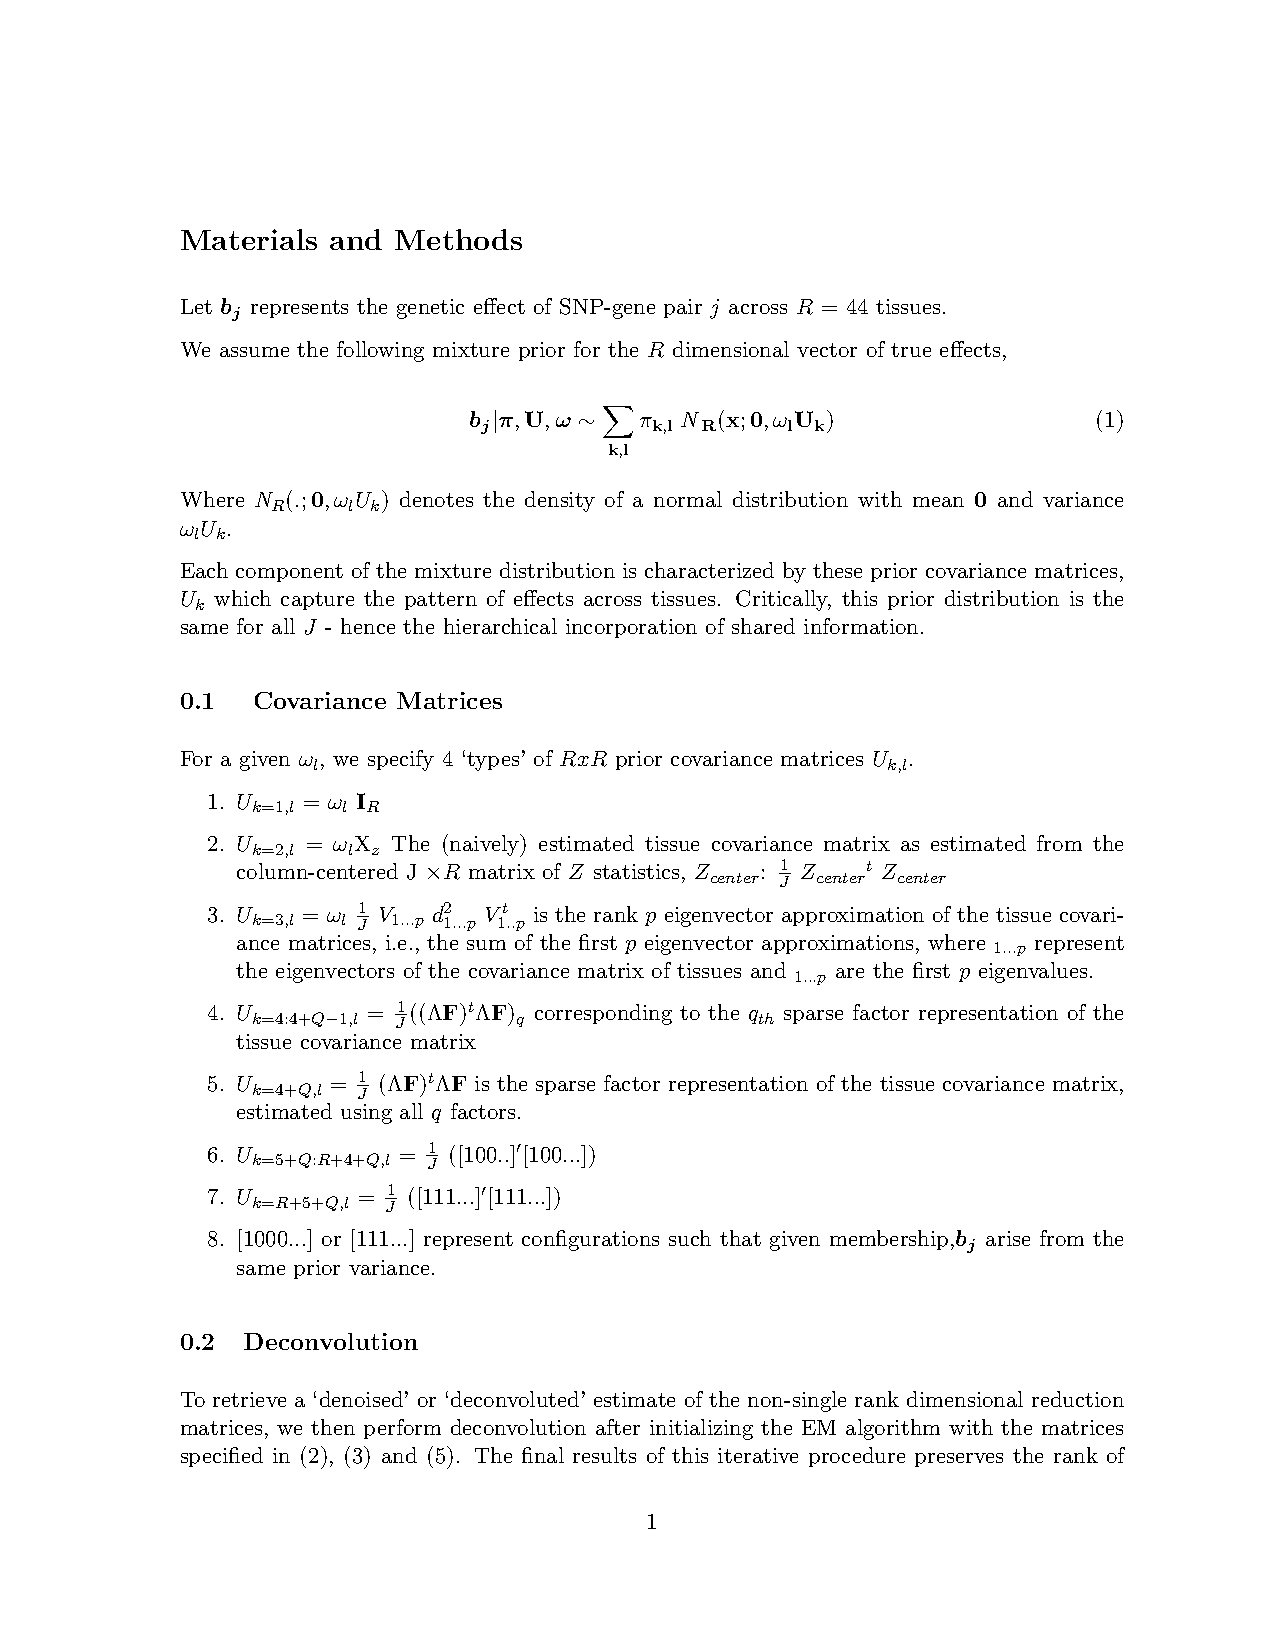
\includegraphics[]{Methods.pdf}

We aim to report posterior quantities for a given gene-snp pair $\textbf{j}$. We know that for a single multivariate {\it Normal}  the posterior on  $\bm{b} | U$ is  simply: 

\begin{equation}
\[
\bm{b} | \hat{\bm{b}} \sim {\it N}_R(\bm{\tilde{\mu}}, \tilde{U})
\]
\end{equation}

where:
\begin{itemize}
\item $\bm{\tilde{\mu}}= \tilde{U}(\hat{V}^{-1} \hat{\bm{b}})$
\item $ \tilde{U} = ({U}^{-1} + \hat{V}^{-1})^{-1}$.
\end{itemize}

Let us concatenate the list of all KxL combinations of prior covariance matrices $U_{k}$ and their scaling parameters $\omega_{l}$ into a KxL list and assign this length K for simplicity of notation.

Now each $U_{k}$ imparts information about both $\emph{scale}$ and $\emph{direction}$
. 
Furthermore, a mixture-multivariate normal prior and a normal likelihood yields a mixture multivariate posterior, where the final posterior distribution is simply a weighted combination of multivariate normal distributions, where for each gene-snp pair $\textbf{j}$ is now characterized by it's posterior mean $\tilde{\bm{\mu}}_{jk}$ and covariance  $\tilde{U}_{jk} = (U_{k}^{-1} + \hat{V}_{j}^{-1})^{-1}$.

\begin{equation}
\begin{aligned}
  \label{eq:mixpost}
\bm{b}_{j} | \hat{\bm{b}_{j}}, \hat{V}_{j}, \hat{\bm{\pi}} 
%&= \sum_{k=1,l=1}^{K,L} \sim {\it N}_R(\bm{\mu}_{1kl}, U_{1kl})%p(\bm{b}_{j} | \hat{\bm{b}}_{j}, \hat{V}_{j}, z_{j}=k,l) 
%p(z=k,l | \hat{\bm{b}}, \hat{V}, \hat{\bm{\pi} }),%v_{j}=1)
 %\\
\sim \sum_{k}^{K}  \tilde \pi_{jk} {\it N}_R (\bf{x};\bm{\tilde{\mu}}_{jk},\tilde{U} _{jk} )%,v_{j}=1) 


\end{aligned}
\end{equation}

Where again, ${\it N}_R(.; \bm{0}, \omega_l U_{k})$ denotes the density of a normal distribution with mean $\bm{\tilde{\mu}}_{k}$ and variance $\tilde{U} _{k}$ and the posterior mixture weight $\tilde \pi_{k}$ is simply 



 \begin{equation}
\tilde \pi_{jk} =\frac{ p(\hat{\bm{b}}_{j}| \hat{V}_{j}, z_{j}=k) \hat \pi_{k} } {\sum_{k=1}^{K} p(\hat{\bm{b}}_{j}| \hat{V}_{j}, z_{j}=k) \hat\pi_{k}}
 \label{eqn:postpi}
\end{equation}

Where $z_{j}=k$ is the latent variable indicator of the component identity and each $\hat\pi_{k}$ represents the Maximum Likelihood Estimate of the prior mixture weights assigned to each component (\ref{eq:pihat}).

\subsection{Reported Quantities}

For every gene-snp pair `j', we aim to report the effect size as the posterior mean, defined as:

\begin{equation}
\begin{aligned}
E(\bm{b}_{j} | \hat{\bm{b}_{j}}, \hat{V}_{j}, \hat{\bm{\pi}})
%&= \sum_{k=1,l=1}^{K,L} \sim {\it N}_R(\bm{\mu}_{1kl}, U_{1kl})%p(\bm{b}_{j} | \hat{\bm{b}}_{j}, \hat{V}_{j}, z_{j}=k,l) 
%p(z=k,l | \hat{\bm{b}}, \hat{V}, \hat{\bm{\pi} }),%v_{j}=1)
 %\\
= \sum_{k}^{K}  \tilde \pi_{k} \bm{\tilde{\mu}}_{k} %,v_{j}=1) 
\end{aligned}
\label{eq:mixmean}
\end{equation}


And the local false sign rate, or posterior probability of incorrectly identifying the sign of the effect for a given tissues `r' as :

\begin{equation}
  \label{eq:lfsr}
\begin{split}
P(b_{jr})= 1-max[{\sum_{k}}p({b_{j,r}}>0|\hat{\bm{b}}_{j}, \hat{V}_{j}, z_{j}=k)\tilde \pi_{k}, {\sum_{k}}p({b_{j,r}}<0|\hat{\bm{b}}_{j}, \hat{V}_{j}, z_{j}=k)\tilde \pi_{jk}]
\end{split}
\end{equation}

For the results section of this paper, we report the  posterior mean ($\ref{eq:mixmean}$) and LFSR ($\ref{eq:lfsr}$) for the `top' snp per gene, but armed with the hierarchical weights (\ref{eq:pihat}) and covariance matrices $\textbf{U}$ the posteriors can be computed for any gene-snp pair.


\section{Results}
\subsection{Demonstrating Features of the Method}

To get a sense of the accuracy of our novel approach to estimating multivariate effects, we simulated two types of data. 

In the first set, in which we expect our method to be superior to both univariate methods and methods in which the configuration approach is utilized, we simulate 50,000 gene-snp pairs, with only 400 representing true signal. This represents roughly 500 genes with 100 snps in cis, $80\%$ of which contain one active QTL. Thus naturally, if the gene contains such a QTL, it is the same QTL among all tissues in which the tissue is active. This puts a dual burden on both features of the method: The small number of true associations present in these simulations tests whether the method accurately encourages small observed effects toward zero while preserving the true signal when it exists. Furthermore, the  multivariate nature of these simulated effects when they exist tests the ability of the method to accurately infer patterns of sharing from the dataset. These true effects are thus simulated from the 'learned' covariance matrices representing $U_{k}$ 2-9, and thus aim to emulate the patterns of sharing present in real biological data. We compare with univariate 'shrinkage' method Ash (Stephens et al, unpublished) as well as the eqtlBMA-lite (Flutre et al, 2013) which uses the singleton and fully consistent (i.e., active in only one tissue, or active with the same effect size in all tissues) configurations to estimate these effects jointly. We call this the 'sharing' (S) scenario. 

One might expect that our method would prove superior only in the setting in which true effects are shared among all tissues, and thus fail in the setting of tissue specificity. Thus, building on the situation above, we add a simulation in which $35\%$ of the true effects are active in only one tissue, according to 5 different patterns of tissue specificity. We call this the 'tissue-specific' (TS) scenario. 

We see that in terms of both power and accuracy, Matrix Ash is superior in both setting to both univariate methods, and to joint analysis under the setting of orthogonal configurations.
\begin{equation}
RMSE \sqrt(\sum_{jr}(b_{jr}-E(b_{jr}|Data)^2))
\end{equation}
\begin{table}[ht]
\caption{Accuracy Comparison: RMSE}
\centering
\begin{tabular}{c c c c}
\hline\hline
Inference Method & MASH & ASH & eqtlBMA-lite \\ [0.5ex] % inserts table %heading
\hline
RMSE_{S}&0.010&0.030&0.047\\
RMSE_{TS}&0.008& 0.025&0.043 \\%&8649
cor.with.truth_{S}&0.99&0.94&0.84\\
cor.with.truth_{TS}&.99&0.94&0.82\\
\hline
\end{tabular}
\label{table:RMSE}
\caption{\textbf{Accuracy Analysis} Here, we compare the ability of matrix ash (`MASH') to capture the true effect size estimates. We compare with univariate-shrinkage method `ASH' and configuration-specific joint approach `eqtl-BMA-lite'. We report the Root Mean Squared Error (RMSE) and the correlation with the truth.}
\end{table}

To demonstrate the ability of Matrix Ash to powerfully capture these accurately estimated effect sizes, we compare the proportion of true associations called significant at a given significance threshold among the three methods. Indeed, Matrix Ash  proves superior to both methods under each condition (i.e., sharing or tissue-specific). 

\texbf{INSERT POWER VS. ACCURACY FIGURE HERE}

In introducing a method to quantify the heterogeneity of effect sizes, we have developed a 'heterogeneity index' which attempts to capture the heterogeneity in magnitude among tissues in which the gene-SNP pair is active. For each gene-snp pair $\textbf{j}$, we normalize its vector of effects $\textbf{b_{j}$ across tissues by the effect which has the maximum absolute value; thus for a fully 'consistent' gene-snp pair in which all the effects are equal in magnitude, the new vector of normalized effects would consist of all ones, and R=44 tissues would be greater than $50\%$ of the maximum effect. By contrast, for a tissue-specific gene-snp pair, the vast majority of effects would be small fraction of the maximum effect and thus the number of tissues greater than $50\%$ of the maximum effect would be 1 (the effect used to normalize). We can apply this heterogeneity index, here deemed 'HI' to the real data, but first wanted to demonstrate the superiority of Matrix Ash in estimating these quantities on simulated data. To quantity the ability of each method to accurately ascertain the heterogeneity, we can compute the heterogeneity index of the real data, and the inferred quantities, and use a modified RMSE:

\begin{equation}
RMSE_{HI} \sqrt(\sum(true_{HI}-estimated_{HI})^2))
\end{equation}

\begin{table}[ht]
\caption{Accuracy Comparison: RMSE}
\centering
\begin{tabular}{c c c c}
\hline\hline
Inference Method & MASH & ASH & eqtlBMA-lite \\ [0.5ex] % inserts table %heading
\hline
HI_{S}&39.38 &40.87 &39.78 \\
HI_{TS}& 39.98& 40.77&39.51\\
\hline
\end{tabular}
\label{table:HETindex}
\end{table}

\subsection{Adaptive Shrinkage: The Multivariate Approach}

To demonstrate the utility of shrinking effect size estimates jointly, we consider the estimated effect sizes vs their observed input summary statistics using our joint (Matrix Ash) and comparing to a univariate shrinkage method (Ash). On simulated data, we can also then plot the estimated effect sizes against the true values,  again comparing among methods. Here, we show the results under the setting of tissue specificity, to analyze the behavior of eQTL of each class. 


\texbf{INSERT TSPEC SIMULATED SCATTERPLOTS HERE}

In both Matrix Ash and univariate methods, values with large standard errors will be shrunk more harshly (Ash, Stephens et al). Comparing estimated Z statistics (i.e., $E(Z_{jr}|Data$) vs the observed 'raw' input values (i.e., $\hat{b_{jr}}$ allows us to understand the behavior of multivariate vs univariate methods once the standard error has been considered. In this simulated data, where there is an abundance of small effects, both univariate and multivariate methods tend to shrink small observed values towards prior mean at $\bm{0}$ as their likelihoods will be maximized by component with small $\omega$. Critically, considering observed Z statistics of the same size, Matrix Ash does not shrink all small values are shrunk to the same extent, due to the power of joint analysis to consider the effects across tissues in inferring the final vector of effect sizes. Thus the method is dually `adaptive' by considering the abundance of both effect sizes and shapes in the overall data-set.  Here, acknowledging consistency, small effects in one tissue will be augmented in the presence of larger effects  other tissues, resulting in dramatic power increases. 

Furthermore, when we plot the estimated effects vs the truth and segregate these effects by class (e.g., active and shared, active and tissue-specific, or null), we see that the correlation among the true and estimated effect $(E(Z|D)$ sizes is much tighter using our multivariate approach. Similarly, truly null effects are shrunk more tightly, due to the fact that in the presence of consistency, small effects across subgroups will lead us to have a high prior belief that an additional small observed effect in that eQTL is also likely to be close to 0. Importantly, tissue-specific QTLs are still captured using our joint approach, demonstrating that if tissue-specific patterns exist in the data, our prior belief will capture this phenomenon and accordingly our posterior estimates will reflect the underlying tissue-specific nature at a given tissue-specific SNP.

Together, these results demonstrate the tremendous power increase of using a multivariate method and the accuracy of estimating patterns of sharing from the data rather than imposing forced configurations which fail to capture the heterogeneity of effect sizes among tissues.


\section{Real Data}

Now, we consider the results of our analysis, when applied to the GTEX data set. After estimating the covariance matrices from the strongest Z statistics in the data, thus demonstrating the strong underlying 'true patterns' of sharing in the data and adding the qualitatively specific configurations, we then inferred the relative frequency of each pattern of sharing and corresponding effect sizes from a large sample of 40,000 gene-snp pairs. Here, we report the analysis on the top SNP for each of 16,069 genes, where the 'top' snp is defined as the SNP with the largest effect size in absolute value across tissues. As described above and demonstrated in simulations, in the setting of an abundance of small effects in data set, we  tends to shrink small z statistics towards the prior mean at 0. It should be noted that this is a result specific to a particular data set, and in that sense 'adaptive' - indeed, if small effects were rare and large effects abundant, such shrinkage would not occur. 

But perhaps more importantly, the striking increase in power when compared to univariate methods is noted. There are a total of 44 tissues x 16,069 gene-snp pair associations considered, or 707,036 total tissue-level effect size coefficients. At an $lfsr$ threshold of 0.05, we identify 393,414 significant snp-gene-tissue effects ($b_{jr}$). Using estimates shrunk according to a univariate approach (again, Ash),  we identify only 91,755, meaning that using univariate methods we would be confident our ability to identify the sign in only $13\%$ of cases, while using our joint procedure for estimating effects, we would confidently argue the SNP has a non-zero effect for a gene in a particular tissue over half $(55\%)$ of the time. As described, this tremendous increase in power arises from the fact that in the presence of  a data set possessing consistency, as learned by the hierarchical model, small effects in the presence of a gene containing large effects in alternative tissues will be augmented to reflect such consistency, thus increasing our confidence in its size and direction. While the number of associations capture is slightly greater using the BMA lite approach, we note that the likelihood of the data set under this model is much much worse ($-1298672$ vs $-1267997.5$, see supplementary data 'Testing and Training' procedure). Indeed, eQTLBMA would put the vast majority of the prior weight on the fully 'consistent' configuration ($\hat{\pi}}$ figure, as SNPs demonstrating activity across all tissues, regardless of how heterogeneous among subgroups, are forced into this configuration. Simulations above demonstrate the lack of accuracy arising from such an approach.

\textbf{SHOW REAL DATA SCATTERPLOT}

\begin{table}[ht]
\caption{Power Comparison}
\centering
\begin{tabular}{c c c c}
\hline\hline
Metric & LFSR_{Matrix Ash} & LFSR_{ASH}&eQTL-BMALite \\ [0.5ex] % inserts table %heading
\hline
Significant $\bf{b}_{jr}$ $\leq$ 0.05%&202087
&393414 & 91,755&401552\\
%$\bf{b}_{jr}$ significant in other not in MASH %&8649
&NA&1447 \\
%$\bf{b}_{jr}$ significant in MASH not in other %&199976
&NA&303106 \\[1ex]
\hline
\end{tabular}
\label{table:power}
\caption{\textbf{Power} Restricting our analysis to thresholding by local false sign rates, we can quantify the number of associations we identify at a given local false sign rate threshold using the original summary statistics and posterior means computed using multivariate Matrix Ash and Univariate Ash. We can see that Matrix Ash calls nearly twice and 4 times as many associations significant when compared to univariate approach, and is comparable to less-accurate joint approach}
\end{table}


\textbf{SHOW $\hat{\pi} barplot in MASH vs BMAlite}

To further contrast our approach with existing joint methods on this data-set, consider a two-tissue example, in which a configuration type approach recognizes only patterns constrained to lie along the x and y axis or along the x-y line. Matrix ash allows for patterns which show consistently larger effects in one tissue over another, with varying amounts of correlation among tissues. In these example from real data, we can see that while SNPS of the green, blue and yellow class appear consistently active in both tissues plotted (Brain and Muscle), the blue and yellow effects have consistently larger effects in Skeletal Muscle than brain, while SNPs of the green class show the reverse. Similarly, SNPS of the yellow close show only loose correlation among the pair of tissues, while SNPs of the green class show strong prediction of activity in one from activity in the other.  Similarly, we can see that SNPS of the pink class tend to show tissue-specificity in Whole Blood relative to testis, while SNPs of the black class show tissue specificity in testis relative to whole blood.

\textbf{SHOW COLORED SCATTERPLOT}

\subsection{ A qualitative description of heterogeneity in the GTEX data}

Indeed, from the prior weight assigned to the 'learned matrices' above coupled with the simulation results in the previous sections, we can see that Matrix ASH is able to accurately parse shared configurations. Focusing on the two predominant patterns, we see that  Here we examine several examples with a high posterior probability of arising from this particular component while the learned matrix $U_{k}$ = 3 seems to capture gene-snp pairs with large, correlated effects in brain, matrix $U_{k}$ = 2 captures SNPs with small effects in brain and larger effects in thyroid and transformed cell-types (e.g., fibroblasts, lymphocytes). The lower which rank high in importance (e.g., $U_{k} 5 and $U_{k}$ = 9) show somewhat tissue specific (i.e., high prior variance in only one tissue-type) effects in testes and whole blood, consistent with our conclusions that whole blood and testes indeed demonstrate an abundance of tissue-specific gene-snp pairs.


\subsection{Examples of strong loading on Uk3, Uk9 and eQTL-BMA lite}


\textbf{Uk3: Captures correlation in sign, quantitative heterogeneity in magnitude along diagonal emphasizes the utility of continuous approach}
In this particular example, strong effects in brain matching an underlying pattern of shared effects among brain tissue is well-captured by the data and thus allows this gene-snp pair to find its true match. brain effect sizes thus borrow strength from one another, and the posterior estimates tend to nudge the brains towards a consistent, shared effect. Similarly, an overall tendency towards consistency tends to 'flip' erratic off directions towards the prevailing positive direction.

%Flip 'erratic' off directions, but maintain ability to recognize when we lack confidence in sign of the effect
\textbf{Uk 9: Quantitative specificity in magnitude in testes/Whole Blood}
In this example, though this particular pattern captures correlation in sign among all tissues, the quantitative heterogeneity is reflected in the intensity of the banding along the diagonal, and thus introduces the idea of quantitative specificity - e.g., that a SNP can be modestly 'active' in all tissues though to dramatically different degrees. here, though this matrix was learned (and not forced, as in eQTLBMAlite) from the data, the pattern of quantitative tissue specificity in testes and whole blood is evident. Again, erratic, off-directions are flipped in sign.

Lastly, the inclusion of the eQTLBMA lite configurations (in which the SNP has a non-zero effect in only one tissue) coupled with the learned patterns of tissue specificity evident in matrices $U_{k}5-9$ serve to allow the preservation of qualitatively specific effects. Here, we show a gene-snp pair demonstrating high loading on one of the eqtlbma-lite configuration matrices - indeed, we reject the significance of the effect size estimates in all tissues but testes, a pattern consistent with the presence of tissue-specificity described below.


\subsection{Tissue Specificity}

One of the criticisms of a joint approach might be its loss of tissue-specificity. That is, by considering effects across subgroups in estimating the effect size, one might lose sight of tissue specific activity when it exists. Here, we demonstrate our ability to recognize such specificity both quantitatively (through learned patterns of sharing which specify consistently larger effects in one tissue over others) and qualitatively (through forced prior effect size mass on 0).  For each tissue, we can ask how many gene-snp pairs meet a given significance threshold in that tissue alone. 
\textbf{NUMBER OF QTL PER TISSUE PLOT}

Furthermore, tissue specific eQTL demonstrate the smoothing feature of this joint shrinkage approach: for gene SNP pairs which demonstrate strong effects in only one tissue, the weaker erratic tissue are shrunk towards the prior mean at 0, resulting in a tissue specific smoothing.

\textbf{TISSUESPECIFIC SMOOTHING PLOT}

\subsection{Quantifying Heterogeneity}


Armed with a vector of effect size estimates across 44 tissues, we can move beyond asking in how many tissues is a given gene-snp pair significant, and ask about the relationship in effect size and direction among tissues in which the gene-snp pair is active. From a biological standpoint, we might consider think that effects of a different sign are rare. Similar to the heterogeneity index described in the simulation framework above which attempted to describe heterogeniety in magnitude, we can plot the number of tissues in which the sign is differ than the effect with maximum absolute value. Considering this results with and without the inclusion of the brain tissues, which appear to behave as a strongly correlated group, we observe several phenomenon. The majority of gene-snp pairs are consistent in sign (indeed, only about $20\%$ of genes show two significant effects of a different sign when including brain, and even fewer $(14.8\%)$ when excluding brains) and removing brains from our analysis tends to push us towards consistency, suggesting that brain appears to behave as a large tissue-specific entity.



\textbf{Sign Heterogeneity Hist}

Furthermore, we can now quantify the heterogeneity index in magnitude described in the simulation framework above, and ask, for each gene, in how many tissues is the effect a certain  proportion, suppose $50\%$, of the maximum effect? Again, homogenous genes will tend to be featured at the right of the distribution, with the majority of their tissues effect sizes similar in magnitude, while heterogneous genes will be featured towards the left, with tissue-specific genes at the extreme left. Again, excluding brain form the analysis tends to nudge us towards a belief in consistency. We can also consider how many gene-snp-tissue (i.e., $b_{jr}$) effects are greater than $50\%$ of the maximal value for the gene (gene `j'): such a contrast is evident here as 

Taken together, these results suggest the presence of consistency in sign in our data set, and a bimodal distribution of heterogeneity in magnitude.
\begin{table}[htbp]
\caption{Heterogeneity Comparison}
\centering
\begin{tabular}{c c c c}
\hline\hline
Data & All Tissues  & No Brains  \\ [0.5ex] % inserts table %heading
\hline
%Consistent in Sign (normalized value $>$ 0): E(Z$\mid$D)$ &0.833&0.880 \\
%E(DifferentSign (no threshold)&0.906 ( 0.87 no brains) &0.597&0.481\\
E(DifferentSignPosteriorMean$\mid$ LFSR$\leq$0.05)&0.802&0.852\\
E(At least 50\% max value) &0.354&0.449\\
%Sign Change &0&0.184&0.179\\[1ex]
\hline
\end{tabular}
\label{table:nonlin}
\caption{\textbf{Heterogeneity Analysis} At a given significance threshold, we can ask how many gene-pairs contain effects of different signs across tissues. At an arbitrary LFSR threshold of 0.05 for instance, we note that $80\%$ of genes are homogenous in sign when all tissues are considered. Excluding brains from our analysis, this rises to $85\%$. To evaluate consistency in magnitude, we can ask how many gene-snp-tissue effects are greater than $50\%$ of the maximal effect across tissues for the pair. Again, we see that excluding brains from our analysis tends to push this towards consistency.}
\end{table}

\textbf{Magnitude Heterogeneity Index}

Attempting to understand which genes tend to behave the most homogenously or heterogeneously, we can plot the value used to normalize each gene, e.g., the 'maximum' effect size across tissue of the gene, against the normalized values. We can see that if a large effect is present, it tends to be in the presence of homogenous effects across the board, while small normalizing effects tend to be in the presence of effects that are more variable in sign and magnitude. Furthermore, aggregating the gene-snp pairs at a given heterogeneity index and classifying them by the effect used to normalize (e.g., the 'max effect') we can see that gene-snp pairs with greater Heterogeneity indices tend to have larger effects.

\textbf{Insert BIPLOT}
\textbf{Insert Median MAX EFFECT by HI Index}
\textbf{Insert }




%In how many genes do there exists effects of a different sign? 
%9,597 (59.7%) vs 7,723 (48.1%)
% What about effects at a given significance threshold?
%3,180 with brain includes (19.8%), 2,377 no brain at an LFSR threshold of 0.05 ( 14.8%)
%Gene.snp.tissue.effects (i.e., b.j.r)
%With brains: Proportion b.j.r norm>0: 83.3 % Without brains: 88%
%Proportion b.j.r norm>50%: 35.4 vs 44.9%


\section{Testing and Training}

In order to determine the optimal number and rank of the covariance matrices, we divide our data set into a training and test data set, each containing 8000 genes.

In the training set, we proceed as above: choosing the top SNP for each of the 8000 genes, creating a list of covariance matrices through deconvolution and grid selection of these top 'training gene-snp' pairs. 

Then, within the training data, we similarly choose a random set of gene-snp pairs (restricting our analysis to genes contained in the training set. Again, we choose 20,000 random-gene snp pairs and use the EM algorithm to learn the mixture proportions $\pi$  from this data set.

We then use the KxL vector of $\pi$ from the training set to estimate the log likelihood of each data point in the test data set. If our model is 'overfit' to the training data set, than a larger number of covariance matrices may actually decrease the test log-likelihood. 

I found that the K=1188 set of covariance matrices containing the Identity, the denoised empirical covariance matrix, rank 5 SFA approximation and rank 3 SVD approximation as well as 5 single-rank SFA factors and the 45 $eqtl.bma.lite$ configurations maximized this likelihood.




\section{Training and Testing Procedure: Estimating Hierarchical Weights}

We wish to choose the model which best maximizes the probability of observing the data set. 

Incomplete Data likelihood:
%Here, the total likelihood of the test data set over $K$ components: 

\begin{equation}
L(\bm\pi;{\hat{\bm{b}})} = \prod_{j=1}^J \sum_{k}^{K} \pi_{k} P(\hat{\bm{b_{j}}} | z_{j}=k)
\end{equation}

\begin{itemize}
\item  To estimate the hierarchical prior weights $\pi_{k}$: compute the likelihood at each each gene snp pair $j$ by evaluating the probability of observing $\bm{\hat{b}_{j}}$ given that we know the true $\bm{b_{j}}$ arises from component $k$
\item  Use the EM algorithm to estimate the optimal combination of weights: How often does this particular covariance matrix occur in the data?
\end{itemize}

We then use these weights to estimate the test set log likelihood.

% Results and Discussion can be combined.

%Nulla mi mi, venenatis sed ipsum varius, Table~\ref{table1} volutpat euismod diam. Proin rutrum vel massa non gravida. Quisque tempor sem et dignissim rutrum. Lorem ipsum dolor sit amet, consectetur adipiscing elit. Morbi at justo vitae nulla elementum commodo eu id massa. In vitae diam ac augue semper tincidunt eu ut eros. Fusce fringilla erat porttitor lectus cursus, vel sagittis arcu lobortis. Aliquam in enim semper, aliquam massa id, cursus neque. Praesent faucibus semper libero.
%
%
%\begin{table}[!ht]
%\begin{adjustwidth}{-2.25in}{0in} % Comment out/remove adjustwidth environment if table fits in text column.
%\caption{
%{\bf Table caption Nulla mi mi, venenatis sed ipsum varius, volutpat euismod diam.}}
%\begin{tabular}{|l|l|l|l|l|l|l|l|}
%\hline
%\multicolumn{4}{|l|}{\bf Heading1} & \multicolumn{4}{|l|}{\bf Heading2}\\ \hline
%$cell1 row1$ & cell2 row 1 & cell3 row 1 & cell4 row 1 & cell5 row 1 & cell6 row 1 & cell7 row 1 & cell8 row 1\\ \hline
%$cell1 row2$ & cell2 row 2 & cell3 row 2 & cell4 row 2 & cell5 row 2 & cell6 row 2 & cell7 row 2 & cell8 row 2\\ \hline
%$cell1 row3$ & cell2 row 3 & cell3 row 3 & cell4 row 3 & cell5 row 3 & cell6 row 3 & cell7 row 3 & cell8 row 3\\ \hline
%\end{tabular}
%\begin{flushleft} Table notes Phasellus venenatis, tortor nec vestibulum mattis, massa tortor interdum felis, nec pellentesque metus tortor nec nisl. Ut ornare mauris tellus, vel dapibus arcu suscipit sed.
%\end{flushleft}
%\label{table1}
%\end{adjustwidth}
%\end{table}
%
%
%
%\subsection*{\lorem\ and \ipsum\ Nunc blandit a tortor.}
%
%Maecenas convallis mauris sit amet sem ultrices gravida. Etiam eget sapien nibh. Sed ac ipsum eget enim egestas ullamcorper nec euismod ligula. Curabitur fringilla pulvinar lectus consectetur pellentesque. Quisque augue sem, tincidunt sit amet feugiat eget, ullamcorper sed velit. Sed non aliquet felis. Lorem ipsum dolor sit amet, consectetur adipiscing elit. Mauris commodo justo ac dui pretium imperdiet. Sed suscipit iaculis mi at feugiat. 
%
%\subsection*{Sed ac quam id nisi malesuada congue.}
%
%Nulla mi mi, venenatis sed ipsum varius, volutpat euismod diam. Proin rutrum vel massa non gravida. Quisque tempor sem et dignissim rutrum. Lorem ipsum dolor sit amet, consectetur adipiscing elit. Morbi at justo vitae nulla elementum commodo eu id massa. In vitae diam ac augue semper tincidunt eu ut eros. Fusce fringilla erat porttitor lectus cursus, vel sagittis arcu lobortis. Aliquam in enim semper, aliquam massa id, cursus neque. Praesent faucibus semper libero.
%
%% Please do not create a heading level below \subsection. For 3rd level headings, use \paragraph{}. 
%\subsection*{Subsection 1}
%Nulla mi mi, venenatis sed ipsum varius, volutpat euismod diam. Proin rutrum vel massa non gravida. Quisque tempor sem et dignissim rutrum. Lorem ipsum dolor sit amet, consectetur adipiscing elit. Morbi at justo vitae nulla elementum commodo eu id massa. In vitae diam ac augue semper tincidunt eu ut eros. Fusce fringilla erat porttitor lectus cursus, vel sagittis arcu lobortis. Aliquam in enim semper, aliquam massa id, cursus neque. Praesent faucibus semper libero.
%
%\subsection*{Subsection 2}
%\paragraph{3rd Level Heading.} Nulla mi mi, venenatis sed ipsum varius, volutpat euismod diam. Proin rutrum vel massa non gravida. Quisque tempor sem et dignissim rutrum. Lorem ipsum dolor sit amet, consectetur adipiscing elit. Morbi at justo vitae nulla elementum commodo eu id massa. In vitae diam ac augue semper tincidunt eu ut eros. Fusce fringilla erat porttitor lectus cursus, vel sagittis arcu lobortis. Aliquam in enim semper, aliquam massa id, cursus neque. Praesent faucibus semper libero.

\section*{Discussion}
%Nulla mi mi, venenatis sed ipsum varius, Table~\ref{table1} volutpat euismod diam. Proin rutrum vel massa non gravida. Quisque tempor sem et dignissim rutrum. Lorem ipsum dolor sit amet, consectetur adipiscing elit. Morbi at justo vitae nulla elementum commodo eu id massa. In vitae diam ac augue semper tincidunt eu ut eros. Fusce fringilla erat porttitor lectus cursus, vel sagittis arcu lobortis. Aliquam in enim semper, aliquam massa id, cursus neque. Praesent faucibus semper libero.
%
%\subsection*{\lorem\ and \ipsum\ Nunc blandit a tortor.}
%
%CO\textsubscript{2} Maecenas convallis mauris sit amet sem ultrices gravida. Etiam eget sapien nibh. Sed ac ipsum eget enim egestas ullamcorper nec euismod ligula. Curabitur fringilla pulvinar lectus consectetur pellentesque. Quisque augue sem, tincidunt sit amet feugiat eget, ullamcorper sed velit. 
%
%Sed non aliquet felis. Lorem ipsum dolor sit amet, consectetur adipiscing elit. Mauris commodo justo ac dui pretium imperdiet. Sed suscipit iaculis mi at feugiat. Ut neque ipsum, luctus id lacus ut, laoreet scelerisque urna. Phasellus venenatis, tortor nec vestibulum mattis, massa tortor interdum felis, nec pellentesque metus tortor nec nisl. Ut ornare mauris tellus, vel dapibus arcu suscipit sed. Nam condimentum sem eget mollis euismod. Nullam dui urna, gravida venenatis dui et, tincidunt sodales ex. Nunc est dui, sodales sed mauris nec, auctor sagittis leo. Aliquam tincidunt, ex in facilisis elementum, libero lectus luctus est, non vulputate nisl augue at dolor. For more information, see \nameref{S1_Text}.
%
\section*{Supporting Information}

% Include only the SI item label in the subsection heading. Use the \nameref{label} command to cite SI items in the text.
%\subsection*{S1 Video}
%\label{S1_Video}
%{\bf Bold the first sentence.}  Maecenas convallis mauris sit amet sem ultrices gravida. Etiam eget sapien nibh. Sed ac ipsum eget enim egestas ullamcorper nec euismod ligula. Curabitur fringilla pulvinar lectus consectetur pellentesque.
%
%\subsection*{S1 Text}
%\label{S1_Text}
%{\bf Lorem Ipsum.} Maecenas convallis mauris sit amet sem ultrices gravida. Etiam eget sapien nibh. Sed ac ipsum eget enim egestas ullamcorper nec euismod ligula. Curabitur fringilla pulvinar lectus consectetur pellentesque.
%
%\subsection*{S1 Fig}
%\label{S1_Fig}
%{\bf Lorem Ipsum.} Maecenas convallis mauris sit amet sem ultrices gravida. Etiam eget sapien nibh. Sed ac ipsum eget enim egestas ullamcorper nec euismod ligula. Curabitur fringilla pulvinar lectus consectetur pellentesque.
%
%\subsection*{S2 Fig}
%\label{S2_Fig}
%{\bf Lorem Ipsum.} Maecenas convallis mauris sit amet sem ultrices gravida. Etiam eget sapien nibh. Sed ac ipsum eget enim egestas ullamcorper nec euismod ligula. Curabitur fringilla pulvinar lectus consectetur pellentesque.
%
%\subsection*{S1 Table}
%\label{S1_Table}
%{\bf Lorem Ipsum.} Maecenas convallis mauris sit amet sem ultrices gravida. Etiam eget sapien nibh. Sed ac ipsum eget enim egestas ullamcorper nec euismod ligula. Curabitur fringilla pulvinar lectus consectetur pellentesque.
%
\section*{Acknowledgments}
%Cras egestas velit mauris, eu mollis turpis pellentesque sit amet. Interdum et malesuada fames ac ante ipsum primis in faucibus. Nam id pretium nisi. Sed ac quam id nisi malesuada congue. Sed interdum aliquet augue, at pellentesque quam rhoncus vitae.

\nolinenumbers

%\section*{References}
% Either type in your references using
% \begin{thebibliography}{}
% \bibitem{}
% Text
% \end{thebibliography}
%
% OR
%
% Compile your BiBTeX database using our plos2015.bst
% style file and paste the contents of your .bbl file
% here.
% 


\newpage

%\bibliographystyle{nci}



\bibliography{gtex.bib}

%\begin{thebibliography}{10}
%\bibitem{bib1}
%Devaraju P, Gulati R, Antony PT, Mithun CB, Negi VS. Susceptibility to SLE in South Indian Tamils may be influenced by genetic selection pressure on TLR2 and TLR9 genes. Mol Immunol. 2014 Nov 22. pii: S0161-5890(14)00313-7. doi: 10.1016/j.molimm.2014.11.005
%
%\bibitem{bib2}
%Huynen MMTE, Martens P, Hilderlink HBM. The health impacts of globalisation: a conceptual framework. Global Health. 2005;1: 14. Available: http://www.globalizationandhealth.com/content/1/1/14.
%
%\end{thebibliography}



\end{document}

